\documentclass{article}
\usepackage{amsmath, amssymb, ctex, graphicx, color}
\usepackage[margin=1in]{geometry}
\usepackage{setspace} % 行距控制

\usepackage{titling}\setlength{\droptitle}{-2cm} 
\title{Ch7. Gradient Descent - Section 7.1. Error Surfaces\\
第7章-梯度下降 -- 第7.1节-误差曲面 }
\author{《深度学习基础》课程小组}
% \date{}
 
\begin{document}
\maketitle
\tableofcontents

\setlength{\parindent}{0pt} % 取消首行缩进
\setlength{\parskip}{1.5em} % 设置段落之间的距离

\noindent\rule{\linewidth}{0.4pt}

\section{P1 神经网络的函数逼近能力与参数设定}

In the previous chapter we saw that neural networks are a very broad and flexible class of functions and are able in principle to approximate any desired function to arbitrarily high accuracy given a sufficiently large number of hidden units. 

Moreover, we saw that deep neural networks can encode inductive biases corresponding to hierarchical representations, which prove valuable in a wide range of practical applications. 

We now turn to the task of finding a suitable setting for the network parameters (weights and biases), based on a set of training data.

{\color{red}
翻译：

在前一章中我们看到，神经网络是一类非常广泛且灵活的函数，原则上，只要隐藏单元的数量足够多，它们就能以任意高的精度逼近任何所需的函数。

此外，我们还了解到，深度神经网络能够编码与层级化表示（hierarchical representations）相对应的归纳偏置（inductive biases），而这些偏置在广泛的实际应用中已被证明极具价值。

现在，我们将转向一项新任务：基于一组训练数据，为网络参数（权重和偏置）寻找合适的设定。
}

{\color{blue}
\underline{问：什么是归纳偏置 (Inductive Biases)？}

答：在机器学习中，如果没有预先的假设，模型面对无限多的可能解将无法做出合理预测（这被称为“没有免费午餐定理”）。归纳偏置就是模型为了从有限的数据中进行泛化（推断未见过的数据）而做出的一系列假设或偏好。

通俗理解：就像人类学习时，我们不会把世界看作毫无规律的随机像素，而是会预设“相似的物体通常有相似的属性”或“空间上相邻的事物往往相关”。对于神经网络来说，它的归纳偏置就是它倾向于学习什么样的模式。例如，卷积神经网络（CNN）的归纳偏置是“平移不变性”（即不管猫出现在图片的左上角还是右下角，它都是猫）。

\underline{问：什么是层级化表示 (Hierarchical Representations)？}

答：这是深度学习（尤其是多层神经网络）的核心特征，指的是数据特征被组织成从低级到高级、从简单到复杂的层次结构。

通俗理解：以人脸识别为例，神经网络的底层可能只提取简单的边缘、线条和颜色块；中间层会将这些线条组合成眼睛、鼻子等局部器官；而高层则会将这些器官组合成一张完整的人脸。这种层层递进、由简入繁的特征提取方式，就是层级化表示。它使得模型能够高效地理解复杂的数据结构。

实验：结合一个具体的例子（比如MNIST手写数字识别），把这两个概念串起来。理论落到实际数据上会更容易理解。
}

\noindent\rule{\linewidth}{0.4pt}

\section{P2 基于梯度的误差函数优化}

As with the regression and classification models discussed in earlier chapters, we choose the model parameters by optimizing an error function. 

We have seen how to define a suitable error function for a particular application by using maximum likelihood. 

Although in principle the error function could be minimized numerically through a series of direct error function evaluations, this turns out to be very inefficient. 

Instead, we turn to another core concept that is used in deep learning, which is that optimizing the error function can be done much more efficiently by making use of gradient information, in other words by evaluating the derivatives of the error function with respect to the network parameters. 

This is why we took care to ensure that the function represented by the neural network is differentiable by design. 

Likewise, the error function itself also needs to be differentiable.

{\color{red}
翻译：

与前面章节中讨论的回归和分类模型一样，我们通过优化一个误差函数来选择模型参数。

我们已经了解了如何利用最大似然法（maximum likelihood）为特定应用定义一个合适的误差函数。

虽然从原理上讲，我们可以通过一系列直接评估误差函数值的方式来对其进行数值最小化，但事实证明这种做法效率非常低。

相反，我们转向深度学习中另一个核心概念，即：通过利用梯度信息 — — 换句话说，通过计算误差函数对网络参数的导数 — — 可以更加高效地优化误差函数。

这就是为什么我们要确保神经网络所表示的函数在设计上就是可微的。

同样地，误差函数本身也必须是可微的。
}

{\color{blue}
\underline{问：如何用 Maximum Likelihood 构造误差函数？}

答：最大似然的核心思想是：找到一组参数，使得在这组参数下，我们观测到当前训练数据的概率（似然）最大。

具体步骤如下：

1. 写出似然函数：假设训练数据集为 $\{(x_1, t_1), (x_2, t_2), \dots, (x_N, t_N)\}$，在参数 $\mathbf{w}$ 下，假设各样本独立同分布，则似然函数为所有样本概率的乘积：
$$L(\mathbf{w}) = \prod_{n=1}^{N} p(t_n | x_n, \mathbf{w})$$

2. 取对数：将乘积转化为求和，得到对数似然函数，方便计算：
$$\ln L(\mathbf{w}) = \sum_{n=1}^{N} \ln p(t_n | x_n, \mathbf{w})$$

3. 转化为误差函数：最大化对数似然等价于最小化负对数似然（Negative Log-Likelihood, NLL），这就自然得到了误差函数：
$$E(\mathbf{w}) = -\ln L(\mathbf{w}) = -\sum_{n=1}^{N} \ln p(t_n | x_n, \mathbf{w})$$

常见例子：\\
对于回归问题（假设噪声为高斯分布），最大似然导出的误差函数就是均方误差（MSE）。\\
对于二分类问题（假设输出服从伯努利分布），最大似然导出的误差函数就是交叉熵损失（Cross-Entropy Loss）。


\underline{问：什么是 Direct Error Function Evaluations？}

Direct error function evaluations（直接误差函数评估）指的是：不使用梯度信息，仅仅通过反复"代入参数值 → 计算误差函数的数值"来寻找最小值。

可以把它想象成一种"盲搜"策略：

你随机选一组参数，算一下误差是多少；\\
再换一组参数，再算一下；\\
比较哪个误差更小，逐步逼近最小值。

典型的例子包括网格搜索（Grid Search）、随机搜索（Random Search），甚至一些无导数优化方法（如 Nelder-Mead 单纯形法）。

为什么它效率很低？ 因为神经网络的参数量通常非常大（动辄数万到数百万个权重），在高维空间中逐点评估函数值，就像蒙着眼睛在一片巨大的山谷里找最低点 — — 每次只能"踩一脚"感受一下脚下的高低，完全不知道哪个方向是下坡。而利用梯度信息（即导数），就好比知道了脚下山坡的倾斜方向，可以直接朝着下坡方向大步前进，效率天差地别。

这也是为什么深度学习中几乎都依赖基于梯度的优化方法（如梯度下降、Adam 等），而不是直接暴力搜索。
}

\noindent\rule{\linewidth}{0.4pt}

\section{P3 反向传播算法的高效导数计算}

The required derivatives of the error function with respect to each of the parameters in the network can be evaluated efficiently using a technique called backpropagation, which involves successive computations that flow backwards through the network in a way that is analogous to the forward flow of function computations during the evaluation of the network outputs.

{\color{red}
翻译：

误差函数对网络中各个参数的导数，可以利用一种称为反向传播（backpropagation）的技术来高效计算。该技术涉及一系列连续的计算过程，这些计算在网络中由后向前传递，其方式类似于在评估网络输出时函数计算的前向传递过程。
}

{\color{blue}
\underline{问：导数是如何高效计算的？}

答：导数之所以能高效计算，核心在于反向传播算法巧妙地运用了微积分中的链式法则（Chain Rule），并利用了动态规划（Dynamic Programming）的思想来避免重复计算。

具体的高效计算机制可以分为以下几个关键点：

1. 链式法则的逐层分解

在神经网络中，误差函数是层层嵌套的复合函数。根据链式法则，一个复杂函数的导数可以拆解为一系列简单局部导数的乘积。反向传播将全局导数的计算分解为：
$$\frac{\partial \text{误差}}{\partial \text{某层参数}} = \frac{\partial \text{误差}}{\partial \text{该层输出}} \times \frac{\partial \text{该层输出}}{\partial \text{该层输入}} \times \frac{\partial \text{该层输入}}{\partial \text{该层参数}}$$

2. 避免重复计算（核心高效点）

如果不使用反向传播，而是对每个参数单独求导，由于很多中间变量（如某一层的输出）被多个后续参数共享，会导致极其庞大的重复计算。

反向传播的做法是从输出层向输入层逐层回传“误差信号”（即局部梯度）。当计算到某一层时，该层对最终误差的贡献（即 $\frac{\partial \text{误差}}{\partial \text{该层输出}}$）已经被上一层计算好并传过来了。这一层只需要把它与自己的局部导数相乘，就能直接得到该层所有参数的梯度，然后继续传给下一层。

3. 前向与后向的对称性

正如原文所述，这个过程是前向计算的“镜像”：

前向传播（Forward Pass）：输入数据 $\rightarrow$ 逐层计算 $\rightarrow$ 得到预测结果 $\rightarrow$ 计算误差。在这个过程中，所有中间变量（如激活值）都被保存下来。

反向传播（Backward Pass）：从误差开始 $\rightarrow$ 利用前向保存的中间变量 $\rightarrow$ 逐层往回乘局部导数 $\rightarrow$ 得到所有参数的梯度。

总结：
通过这种“前向算值，后向算导”的机制，反向传播将计算整个网络梯度的时间复杂度控制在了与“一次前向传播”相当的水平（大约只是前向传播的两倍计算量）。相比于暴力求导或数值微分，它将原本呈指数级爆炸的计算量降维成了线性级别，这正是深度学习得以训练庞大模型的根本原因。

实验：用一个简单的两神经元网络，手动走一遍前向传播和反向传播的具体计算过程。
}

\noindent\rule{\linewidth}{0.4pt}

\section{P4 泛化能力与正则化的重要性}

Although the likelihood is used to define an error function, the goal when optimizing the error function in a neural network is to achieve good generalization on test data. 

In classical statistics, maximum likelihood is used to fit a parametric model to a finite data set, in which the number of data points typically far exceeds the number of parameters in the model. 

The optimal solution has the maximum value of the likelihood function, and the values found for the fitted parameters are of direct interest. 

By contrast, modern deep learning works with very rich models containing huge numbers of learnable parameters, and the goal is never simply exact optimization. 

Instead, the properties and behaviour of the learning algorithm itself, along with various methods for regularization, are important in determining how well the solution generalizes to new data.

{\color{red}
翻译：

尽管似然函数被用来定义误差函数，但在神经网络中优化误差函数的目标，是为了在测试数据上实现良好的泛化能力。

在经典统计学中，最大似然法被用于将参数模型拟合到有限的数据集上，在这种情况下，数据点的数量通常远远多于模型中的参数数量。

最优解对应于似然函数的最大值，而拟合得到的参数值本身具有直接的参考价值。

相比之下，现代深度学习使用的是包含海量可学习参数的极其复杂的模型，其目标从来都不是简单的精确优化。

相反，学习算法本身的属性和行为，以及用于正则化的各种方法，在决定模型对新数据的泛化能力方面起着至关重要的作用。
}

{\color{blue}
核心思想解析：

这段话点出了经典统计学与现代深度学习在优化理念上的根本差异：

经典统计学：数据多、参数少。目标是“精确拟合”（Exact Optimization），找到那个让似然最大化的唯一最优解。

现代深度学习：参数极多（甚至多于数据量）。如果一味追求训练集上的精确优化，极易导致过拟合（Overfitting）。因此，深度学习更看重模型的泛化能力（Generalization）。为了防止模型死记硬背训练数据，必须依赖算法本身的特性（如随机梯度下降的隐式正则化）以及显式的正则化手段（如 Dropout、权重衰减等）来约束模型。

% 要不要我展开讲讲常见的正则化方法（如L2权重衰减、Dropout），以及它们是如何从优化角度提升泛化能力的？

}

\noindent\rule{\linewidth}{0.4pt}
 
%7.1. Error Surfaces
\section{P5 权重空间与误差曲面的几何直观}

Our goal during training is to find values for the weights and biases in the neural network that will allow it to make effective predictions. 

For convenience we will group these parameters into a single vector $\mathbf{w}$, and we will optimize $\mathbf{w}$ by using a chosen error function $E(\mathbf{w})$. 

At this point, it is useful to have a geometrical picture of the error function, which we can view as a surface sitting over `weight space', as shown in Figure~7.1.

\begin{figure}[h]\centering
    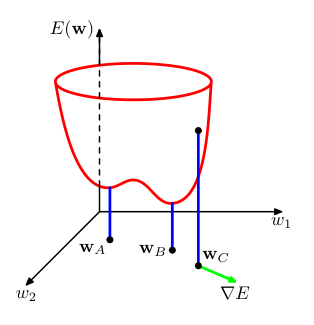
\includegraphics[width=0.4\textwidth]{figure7-1.png}
    \caption{权重空间与误差函数的几何图像}
\end{figure}

Figure 7.1 Caption: Geometrical view of the error function $E(w)$ as a surface sitting over weight space. Point $w_A$ is a local minimum and $w_B$ is the global minimum, so that $E(w_A) > E(w_B)$. At any point $w_C$, the local gradient of the error surface is given by the vector $\nabla E$.

{\color{red}
翻译：

在训练过程中，我们的目标是寻找神经网络中权重和偏置的合适取值，使其能够进行有效的预测。

为了表述方便，我们将这些参数整合为一个单一的向量 $\mathbf{w}$，并通过优化选定的误差函数 $E(\mathbf{w})$ 来对 $\mathbf{w}$ 进行优化。

此时，建立误差函数的几何直观是非常有帮助的。我们可以将误差函数想象为一个覆盖在‘权重空间’之上的曲面，如图 7.1 所示。

图 1：误差函数 $E(w)$ 的几何视角：将其视为覆盖在权重空间之上的曲面。点 $w_A$ 是一个局部极小值点，$w_B$ 是全局极小值点，因此有 $E(w_A) > E(w_B)$. 在任意点 $w_C$ 处，误差曲面的局部梯度由向量 $\nabla E$ 给出。
}

{\color{blue}
\underline{核心概念补充：什么是“权重空间” (Weight Space)？}

结合上一段的内容，这里提到的“权重空间”和“误差曲面”是理解神经网络优化的关键：

权重空间 (Weight Space)：你可以把它想象成一个多维坐标系。如果神经网络有 1000 个参数（权重和偏置），那么权重空间就是一个 1000 维的空间。空间里的每一个“点”，都代表了一组特定的参数组合 $\mathbf{w}$。

误差曲面 (Error Surface)：在这个多维空间中，误差函数 $E(\mathbf{w})$ 就像是地形的高低起伏。参数组合 $\mathbf{w}$ 决定了你在空间中的“水平位置”，而误差值 $E(\mathbf{w})$ 决定了该位置的“海拔高度”。

优化的本质：训练神经网络，在这个几何图景下，就等同于在这个高维地形中寻找海拔最低的山谷（全局极小值或较好的局部极小值）。而前面提到的“反向传播计算梯度”，就相当于蒙着眼睛在山坡上摸索，通过感知脚下的坡度（梯度）来决定往哪个方向迈步（更新参数）。

要不要我展开讲讲这个高维地形里常见的优化难题？比如鞍点（saddle points）和局部极小值（local minima），以及为什么现代优化器（如Adam）能较好地应对它们。
}

\noindent\rule{\linewidth}{0.4pt}
 
%7.1. Error Surfaces
\section{P6 驻点与梯度的数学性质}

First note that if we make a small step in weight space from $\mathbf{w}$ to $\mathbf{w} + \delta\mathbf{w}$ then the change in the error function is given by
\begin{equation}
\delta E \simeq \delta\mathbf{w}^\mathrm{T} \nabla E(\mathbf{w})
\tag{7.1}
\end{equation}
where the vector $\nabla E(\mathbf{w})$ points in the direction of the greatest rate of increase of the error function. 

Provided the error $E(\mathbf{w})$ is a smooth, continuous function of $\mathbf{w}$, its smallest value will occur at a point in weight space such that the gradient of the error function vanishes, so that
\begin{equation}
\nabla E(\mathbf{w}) = \mathbf{0},
\tag{7.2}
\end{equation}
as otherwise we could make a small step in the direction of $-\nabla E(\mathbf{w})$ and thereby further reduce the error. 

Points at which the gradient vanishes are called stationary points and may be further classified into minima, maxima, and saddle points.

{\color{red}
翻译：

首先请注意，如果我们在权重空间中从 $\mathbf{w}$ 向 $\mathbf{w} + \delta\mathbf{w}$ 迈出一小步，那么误差函数的变化量可由下式
\begin{equation}
\delta E \simeq \delta\mathbf{w}^\mathrm{T} \nabla E(\mathbf{w})
\tag{7.1}
\end{equation}
给出，其中向量 $\nabla E(\mathbf{w})$ 指向误差函数增长最快的方向。

假设误差 $E(\mathbf{w})$ 是 $\mathbf{w}$ 的一个平滑、连续函数，那么它的最小值将出现在权重空间中梯度为零的点上，即满足
\begin{equation}
\nabla E(\mathbf{w}) = \mathbf{0},
\tag{7.2}
\end{equation}
因为如果梯度不为零，我们总可以沿着 $-\nabla E(\mathbf{w})$ 的方向迈出一小步，从而进一步降低误差。

梯度为零的点被称为驻点（stationary points），它们还可以进一步分为极小值点（minima）、极大值点（maxima）和鞍点（saddle points）。
}

{\color{blue}
\underline{问：为什么要计算梯度？}

答：这段话奠定了神经网络优化的数学基础，核心解释了为什么我们需要计算梯度以及梯度在寻找最优解时的几何意义：

\begin{itemize}

\item \textbf{公式 (7.1) 的含义（一阶泰勒展开）}：这个公式本质上是一阶泰勒近似。它告诉我们，误差函数的变化量 $\delta E$ 等于步长向量 $\delta\mathbf{w}$ 与梯度向量 $\nabla E(\mathbf{w})$ 的点积。根据向量点积的性质，当 $\delta\mathbf{w}$ 与梯度方向一致时，点积为正且最大（误差增加最快）；当 $\delta\mathbf{w}$ 与梯度方向相反（即 $-\nabla E(\mathbf{w})$）时，点积为负且绝对值最大（误差下降最快）。这就是“梯度下降法”名称的由来。
    
\item \textbf{公式 (7.2) 的含义（极值的一阶必要条件）}：在平滑曲面上寻找最低点，必然要经过坡度为零的地方（就像碗底一定是平的）。$\nabla E(\mathbf{w}) = \mathbf{0}$ 只是找到了“平地”（驻点），但这片平地可能是碗底（极小值）、山顶（极大值）或者是马鞍面（鞍点）。
    
\item \textbf{深度学习中的优化挑战}：在高维权重空间中，鞍点（某些方向上是极小值，另一些方向上是极大值）的数量远远多于局部极小值。这也是为什么在实际训练中，我们不仅依赖梯度（一阶信息）来寻找驻点，还需要借助动量（Momentum）或自适应学习率（如 Adam 优化器）等机制，帮助模型跳出平坦的鞍点区域，继续向更优的解收敛。
\end{itemize}

需要我接着展开讲讲二阶泰勒展开和 Hessian 矩阵吗？它能帮我们区分驻点到底是极小值、极大值还是鞍点。
}

\noindent\rule{\linewidth}{0.4pt}
 
\section{P7 误差曲面的非线性与等效极小值}

We will aim to find a vector $\mathbf{w}$ such that $E(\mathbf{w})$ takes its smallest value. 

However, the error function typically has a highly nonlinear dependence on the weights and bias parameters, and so there will be many points in weight space at which the gradient vanishes (or is numerically very small). 

Indeed, for any point $\mathbf{w}$ that is a local minimum, there will generally be other points in weight space that are equivalent minima. 

For instance, in a two-layer network of the kind shown in Figure~6.9, with $M$ hidden units, each point in weight space is a member of a family of $M!\,2^M$ equivalent points.

{\color{red}
翻译：

我们的目标是寻找一个向量 $\mathbf{w}$，使得误差函数 $E(\mathbf{w})$ 取得最小值。

然而，由于误差函数对权重和偏置参数通常具有高度的非线性依赖关系，因此在权重空间中会存在许多梯度为零（或在数值上非常小）的点。

事实上，对于任何一个局部极小值点 $\mathbf{w}$，权重空间中通常还会存在其他等效的极小值点。

例如，在如图 6.9 所示的具有 $M$ 个隐藏单元的两层网络中，权重空间中的每一个点，都属于一个包含 $M!\,2^M$ 个等效点的集合。
}

{\color{blue}
\underline{问：为什么会有这么多“等效极小值点”？}

答：这揭示了神经网络优化过程中一个非常有趣且重要的现象 — — 对称性（Symmetry）。

1. 排列对称性（$M!$ 的来源）：

在隐藏层中，这 $M$ 个隐藏单元的地位是完全平等的。如果你把其中任意两个隐藏单元的所有输入权重、偏置以及对应的输出权重互换，整个网络的输入输出关系完全不会改变，误差值也一模一样。因为 $M$ 个单元的全排列组合数是 $M!$，所以这就产生了 $M!$ 个等效的解。

2. 符号对称性（$2^M$ 的来源）：

如果隐藏层使用的是奇函数激活函数（例如 $\tanh$ 或 $\tanh$ 的变体 $\arctan$），那么将某个隐藏单元的所有输入权重、偏置以及对应的输出权重同时取反（乘以 $-1$），该单元的输出结果也不会改变。因为每个隐藏单元都有“取反”或“不取反”两种选择，所以又产生了 $2^M$ 种等效状态。

3. 这对训练有什么影响？

这意味着在深度学习中，“全局最优解”并不是唯一的。高维误差曲面上布满了无数个具有相同误差值的“全局极小值山谷”。我们不需要（也不可能）去寻找那个所谓的“唯一绝对最低点”，只要优化算法能帮我们找到其中任意一个足够好的极小值（甚至鞍点附近的平坦区域），模型就能表现出优秀的性能。这也是为什么我们常说深度学习更看重“泛化能力”而非“绝对精确的优化”。

% 要不要我接着展开讲讲梯度下降的具体更新规则？从公式到算法步骤，再到学习率的影响，一步步推下来会很直观。
}

\noindent\rule{\linewidth}{0.4pt}
 
\section{P8 全局极小值与局部极小值}

Furthermore, there may be multiple non-equivalent stationary points and in particular multiple non-equivalent minima. 

A minimum that corresponds to the smallest value of the error function across the whole of $\mathbf{w}$-space is said to be a \emph{global minimum}. 

Any other minima corresponding to higher values of the error function are said to be \emph{local minima}. 

The error surfaces for deep neural networks can be very complex, and it was thought that gradient-based methods might become trapped in poor local minima. 

In practice, this seems not to be the case, and large networks can reach solutions with similar performance under a variety of initial conditions.

{\color{red}
翻译：

此外，还可能存在多个非等效的驻点，特别是多个非等效的极小值点。

在整个 $\mathbf{w}$ 空间中，对应于误差函数最小值的极小值被称为全局极小值（global minimum）。

任何其他对应于较高误差值的极小值被称为局部极小值（local minima）。

深度神经网络的误差曲面可能非常复杂，过去人们曾认为基于梯度的方法可能会陷入较差的局部极小值中。

但在实践中，情况似乎并非如此，在不同的初始条件下，大型网络都能达到具有相似性能的解。
}

{\color{blue}
\underline{问：为什么深度学习不怕“局部极小值”？}

答：这是深度学习优化领域一个非常经典且反直觉的现象。

1. 过去的担忧：在早期的机器学习研究中（比如传统的浅层神经网络），人们普遍认为如果网络初始化不好，梯度下降就会掉进一个很深的“坑”（较差的局部极小值）里爬不出来，导致模型性能很差。

2. 实际的发现：随着网络规模的增大，人们发现这种担忧在大型网络中并不成立。这背后有两个关键的几何原因：

鞍点远多于局部极小值：在极高维的空间中，一个点要成为“局部极小值”，它必须在所有维度上都是极小值。只要有一个维度是上升的，它就是鞍点。随着维度增加，成为真正局部极小值的概率呈指数级下降，因此优化算法遇到的大部分“平地”其实是鞍点，而不是死胡同。

局部极小值的质量都很高：即使真的掉进了局部极小值，研究发现这些极小值对应的误差值往往都非常接近，且通常处于非常平坦的区域（Flat Minima）。平坦的极小值意味着模型对参数的微小扰动不敏感，这恰恰对应着极好的泛化能力。

总结来说：在深度学习中，我们不需要执着于寻找那个绝对最低的“全局极小值”。只要顺着梯度走，找到任何一个足够低且平坦的“局部极小值”，模型就已经非常优秀了。

}

%\subsection{7.1.1 Local quadratic approximation}

\noindent\rule{\linewidth}{0.4pt}
 
\section{P9 误差函数的局部二次近似与泰勒展开}

Insight into the optimization problem and into the various techniques for solving it can be obtained by considering a local quadratic approximation to the error function. 

The Taylor expansion of $E(\mathbf{w})$ around some point $\tilde{\mathbf{w}}$ in weight space is given by
\begin{equation}
E(\mathbf{w}) \approx E(\tilde{\mathbf{w}}) + (\mathbf{w} - \tilde{\mathbf{w}})^\mathrm{T} \mathbf{b} + \frac{1}{2} (\mathbf{w} - \tilde{\mathbf{w}})^\mathrm{T} \mathbf{H} (\mathbf{w} - \tilde{\mathbf{w}})
\tag{7.3}
\end{equation}
where cubic and higher terms have been omitted. 

Here $\mathbf{b}$ is defined to be the \underline{\emph{gradient}} of $E$ evaluated at $\tilde{\mathbf{w}}$
\begin{equation}
\mathbf{b} \equiv \left.\nabla E\right|_{\mathbf{w} = \tilde{\mathbf{w}}}.
\tag{7.4}
\end{equation}

The \underline{\emph{Hessian}} is defined to be the corresponding matrix of second derivatives
\begin{equation}
\mathbf{H}(\tilde{\mathbf{w}}) \equiv \left.\nabla\nabla E(\mathbf{w})\right|_{\mathbf{w} = \tilde{\mathbf{w}}}.
\tag{7.5}
\end{equation}

If there is a total of $W$ weights and biases in the network, then $\mathbf{w}$ and $\mathbf{b}$ have length $W$ and $\mathbf{H}$ has dimensionality $W \times W$. 

From {(7.3)}, the corresponding local approximation to the gradient is given by
\begin{equation}
\nabla E(\mathbf{w}) \approx \mathbf{b} + \mathbf{H}(\mathbf{w} - \tilde{\mathbf{w}}).
\tag{7.6}
\end{equation}

For points $\mathbf{w}$ that are sufficiently close to $\tilde{\mathbf{w}}$, these expressions will give reasonable approximations for the error and its gradient.

{\color{red}
翻译：

通过考虑误差函数的局部二次近似，我们可以深入了解优化问题及其各种求解技术。

误差函数 $E(\mathbf{w})$ 在权重空间中某点 $\tilde{\mathbf{w}}$ 附近的泰勒展开式为：
\begin{equation}
E(\mathbf{w}) \approx E(\tilde{\mathbf{w}}) + (\mathbf{w} - \tilde{\mathbf{w}})^\mathrm{T} \mathbf{b} + \frac{1}{2} (\mathbf{w} - \tilde{\mathbf{w}})^\mathrm{T} \mathbf{H} (\mathbf{w} - \tilde{\mathbf{w}})
\tag{7.3}
\end{equation}
其中省略了三次及更高次的项。

这里 $\mathbf{b}$ 定义为 $E$ 在 $\tilde{\mathbf{w}}$ 处计算的\underline{\emph{梯度（Gradient）}}：
\begin{equation}
\mathbf{b} \equiv \left.\nabla E\right|_{\mathbf{w} = \tilde{\mathbf{w}}}.
\tag{7.4}
\end{equation}

\underline{\emph{海森矩阵（Hessian）}}定义为对应的二阶导数矩阵：
\begin{equation}
\mathbf{H}(\tilde{\mathbf{w}}) \equiv \left.\nabla\nabla E(\mathbf{w})\right|_{\mathbf{w} = \tilde{\mathbf{w}}}.
\tag{7.5}
\end{equation}

如果网络中权重和偏置的总数为 $W$，那么 $\mathbf{w}$ 和 $\mathbf{b}$ 的长度均为 $W$，而 $\mathbf{H}$ 的维度为 $W \times W$。

由公式 (7.3) 可知，梯度的相应局部近似为：
\begin{equation}
\nabla E(\mathbf{w}) \approx \mathbf{b} + \mathbf{H}(\mathbf{w} - \tilde{\mathbf{w}}).
\tag{7.6}
\end{equation}

对于足够接近 $\tilde{\mathbf{w}}$ 的点 $\mathbf{w}$，这些表达式将为误差及其梯度提供合理的近似。

% 需要我接着展开讲讲Hessian矩阵的特征值如何帮助我们判断驻点是极小值、极大值还是鞍点吗？
}

{\color{blue}
\underline{问：解释一下如何从 (7.3) 式得到 (7.6) 式？}

答：从公式 (7.3) 推导到公式 (7.6) 的过程，本质上就是对误差函数的泰勒展开式求梯度（即对向量 $\mathbf{w}$ 求偏导数）。

第一步：写出公式 (7.3)

公式 (7.3) 是误差函数 $E(\mathbf{w})$ 在点 $\tilde{\mathbf{w}}$ 处的二阶泰勒展开：
$$E(\mathbf{w}) \simeq E(\tilde{\mathbf{w}}) + (\mathbf{w} - \tilde{\mathbf{w}})^\mathrm{T} \mathbf{b} + \frac{1}{2} (\mathbf{w} - \tilde{\mathbf{w}})^\mathrm{T} \mathbf{H} (\mathbf{w} - \tilde{\mathbf{w}})$$

第二步：对等式两边同时求梯度 $\nabla E(\mathbf{w})$

我们对等式右边的三项分别关于 $\mathbf{w}$ 求导：

1. 第一项：常数项

$E(\tilde{\mathbf{w}})$ 是在特定点 $\tilde{\mathbf{w}}$ 处计算出的一个固定数值，不包含变量 $\mathbf{w}$。
常数的导数为 0：
$$\nabla [E(\tilde{\mathbf{w}})] = \mathbf{0}$$

2. 第二项：线性项

$(\mathbf{w} - \tilde{\mathbf{w}})^\mathrm{T} \mathbf{b}$ 是关于 $\mathbf{w}$ 的线性函数。
根据向量微积分的基本法则，$\nabla (\mathbf{x}^\mathrm{T} \mathbf{a}) = \mathbf{a}$。因为 $\tilde{\mathbf{w}}$ 是常数向量，$\mathbf{w} - \tilde{\mathbf{w}}$ 对 $\mathbf{w}$ 的导数就是单位矩阵 $\mathbf{I}$，所以：
$$\nabla [(\mathbf{w} - \tilde{\mathbf{w}})^\mathrm{T} \mathbf{b}] = \mathbf{b}$$

3. 第三项：二次型项

$\frac{1}{2} (\mathbf{w} - \tilde{\mathbf{w}})^\mathrm{T} \mathbf{H} (\mathbf{w} - \tilde{\mathbf{w}})$ 是关于 $\mathbf{w}$ 的二次型（Quadratic Form）。
根据向量微积分法则，对于对称矩阵 $\mathbf{H}$，有 $\nabla (\mathbf{x}^\mathrm{T} \mathbf{H} \mathbf{x}) = 2\mathbf{H}\mathbf{x}$。
在这里，令 $\mathbf{x} = \mathbf{w} - \tilde{\mathbf{w}}$，那么：
$$\nabla \left[ \frac{1}{2} (\mathbf{w} - \tilde{\mathbf{w}})^\mathrm{T} \mathbf{H} (\mathbf{w} - \tilde{\mathbf{w}}) \right] = \frac{1}{2} \times 2\mathbf{H}(\mathbf{w} - \tilde{\mathbf{w}}) = \mathbf{H}(\mathbf{w} - \tilde{\mathbf{w}})$$

注：海森矩阵 $\mathbf{H}$ 由二阶偏导数组成，根据克莱罗定理/施瓦茨定理，只要二阶偏导数连续，$\mathbf{H}$ 必然是对称矩阵，因此可以直接应用该法则。

第三步：合并结果

将上述三项的导数相加，我们就得到了误差函数 $E(\mathbf{w})$ 在 $\tilde{\mathbf{w}}$ 附近的梯度近似表达式：
$$\nabla E(\mathbf{w}) \simeq \mathbf{0} + \mathbf{b} + \mathbf{H}(\mathbf{w} - \tilde{\mathbf{w}})$$

整理后即得到公式 (7.6)：
$$\nabla E(\mathbf{w}) = \mathbf{b} + \mathbf{H}(\mathbf{w} - \tilde{\mathbf{w}})$$

总结与意义：

公式 (7.3) 是用一个二次曲面来近似原函数的“高度”（误差值）；

公式 (7.6) 则是用这个二次曲面的切平面斜率来近似原函数的梯度。这在优化算法（如牛顿法 Newton's Method）中极其重要，因为它让我们可以通过求解线性方程组 $\mathbf{H}\Delta\mathbf{w} = -\mathbf{b}$ 来直接“跳跃”到近似极小值点，而不需要像普通梯度下降那样一小步一小步地挪动。

习题：求 $f(x,y)=x^4+y^4$ （或 $f(x,y)=\sin(\pi xy)$） 在点 $(x_0,y_0)=(1,1)$ 附近的二次近似 $g(x,y)$ 的函数表达式。画出这两个函数的图像。
}

\noindent\rule{\linewidth}{0.4pt}
 
\section{P10 海森矩阵与二阶导数信息}

Consider the particular case of a local quadratic approximation around a point $\mathbf{w}^*$ that is a minimum of the error function. 

In this case there is no linear term, because $\nabla E = \mathbf{0}$ at $\mathbf{w}^*$, and {7.3} becomes
\begin{equation}
E(\mathbf{w}) = E(\mathbf{w}^*) + \frac{1}{2} (\mathbf{w} - \mathbf{w}^*)^\mathrm{T} \mathbf{H} (\mathbf{w} - \mathbf{w}^*)
\tag{7.7}
\end{equation}
where the Hessian $\mathbf{H}$ is evaluated at $\mathbf{w}^*$. 

To interpret this geometrically, consider the \underline{\emph{eigenvalue equation}} for the Hessian matrix:
\begin{equation}
\mathbf{H} \mathbf{u}_i = \lambda_i \mathbf{u}_i
\tag{7.8}
\end{equation}
where the eigenvectors $\mathbf{u}_i$ form a complete orthonormal set so that
\begin{equation}
\mathbf{u}_i^\mathrm{T} \mathbf{u}_j = \delta_{ij}.
\tag{7.9}
\end{equation}

We now expand $(\mathbf{w} - \mathbf{w}^*)$ as a linear combination of the eigenvectors in the form
\begin{equation}
\mathbf{w} - \mathbf{w}^* = \sum_i \alpha_i \mathbf{u}_i.
\tag{7.10}
\end{equation}

This can be regarded as a transformation of the coordinate system in which the origin is translated to the point $\mathbf{w}^*$ and the axes are rotated to align with the eigenvectors through the orthogonal matrix whose columns are $\{\mathbf{u}_1,\dots,\mathbf{u}_W\}$. 

By substituting {7.10} into {7.7} and using {7.8} and {7.9}, the error function can be written in the form
\begin{equation}
E(\mathbf{w}) = E(\mathbf{w}^*) + \frac{1}{2} \sum_i \lambda_i \alpha_i^2.
\tag{7.11}
\end{equation}

Suppose we set all $\alpha_i = 0$ for $i \ne j$ and then vary $\alpha_j$, corresponding to moving $\mathbf{w}$ away from $\mathbf{w}^*$ in the direction of $\mathbf{u}_j$. 

We see from {(7.11)} that the error function will increase if the corresponding eigenvalue $\lambda_j$ is positive and will decrease if it is negative. 

If all eigenvalues are positive then $\mathbf{w}^*$ corresponds to a local minimum of the error function, whereas if they are all negative then $\mathbf{w}^*$ corresponds to a local maximum. 

If we have a mix of positive and negative eigenvalues then $\mathbf{w}^*$ represents a saddle point.

{\color{red}
翻译：

考虑在误差函数的极小值点 $\mathbf{w}^*$ 附近进行局部二次近似这一特殊情况。

在这种情况下，由于在 $\mathbf{w}^*$ 处梯度 $\nabla E = \mathbf{0}$，因此不存在线性项，公式 (7.3) 简化为：
\begin{equation}
E(\mathbf{w}) = E(\mathbf{w}^*) + \frac{1}{2} (\mathbf{w} - \mathbf{w}^*)^\mathrm{T} \mathbf{H} (\mathbf{w} - \mathbf{w}^*)
\tag{7.7}
\end{equation}
其中海森矩阵 $\mathbf{H}$ 在 $\mathbf{w}^*$ 处计算。

为了从几何上解释这一点，我们考虑海森矩阵的特征值方程：
\begin{equation}
\mathbf{H} \mathbf{u}_i = \lambda_i \mathbf{u}_i
\tag{7.8}
\end{equation}
其中特征向量 $\mathbf{u}_i$ 构成一个完备的规范正交基，满足：
\begin{equation}
\mathbf{u}_i^\mathrm{T} \mathbf{u}_j = \delta_{ij}.
\tag{7.9}
\end{equation}

现在，我们将 $(\mathbf{w} - \mathbf{w}^*)$ 展开为这些特征向量的线性组合，形式为：
\begin{equation}
\mathbf{w} - \mathbf{w}^* = \sum_{i=1}^{W} \alpha_i \mathbf{u}_i.
\tag{7.10}
\end{equation}

这可以看作是对坐标系的一种变换：将原点平移至点 $\mathbf{w}^*$，并将坐标轴旋转至与特征向量对齐的方向，该旋转由正交矩阵实现，其列向量为 $\{\mathbf{u}_1,\dots,\mathbf{u}_W\}$。

将公式 (7.10) 代入公式 (7.7)，并利用公式 (7.8) 和 (7.9)，误差函数可以写为如下形式：
\begin{equation}
E(\mathbf{w}) = E(\mathbf{w}^*) + \frac{1}{2} \sum_{i=1}^{W} \lambda_i \alpha_i^2.
\tag{7.11}
\end{equation}

假设我们令所有的 $\alpha_i = 0$（$i \ne j$），然后改变 $\alpha_j$ 的值，这相当于使 $\mathbf{w}$ 沿着 $\mathbf{u}_j$ 的方向远离 $\mathbf{w}^*$。

从公式 (7.11) 可以看出，如果对应的特征值 $\lambda_j$ 为正，误差函数将会增加；如果为负，误差函数将会减小。

如果所有特征值均为正，则 $\mathbf{w}^*$ 对应于误差函数的局部极小值；如果所有特征值均为负，则 $\mathbf{w}^*$ 对应于局部极大值；如果特征值中既有正数又有负数，则 $\mathbf{w}^*$ 代表一个鞍点。
}

{\color{blue}
\underline{问：为什么特征值能判断驻点的类型？}

答：我们这里巧妙地用线性代数解决了在高维空间中“盲人摸象”的问题。

1. 坐标系的旋转（解耦）：

在原始的权重空间中，各个维度（参数）之间可能是相互耦合的。但通过特征向量 $\mathbf{u}_i$ 进行坐标变换后，我们找到了误差曲面的“主轴”。在这个新的坐标系下，误差的变化量（公式 7.11）变成了一组互不干扰的独立项 $\frac{1}{2} \lambda_i \alpha_i^2$ 的简单求和。

2. 特征值的几何意义：

每一个特征值 $\lambda_i$ 及其对应的特征向量 $\mathbf{u}_i$，描述了误差曲面在 $\mathbf{u}_i$ 这个特定方向上的“弯曲程度”（曲率）：

$\lambda_i > 0$：曲面在这个方向上像碗底一样向上弯曲（极小值方向）。

$\lambda_i < 0$：曲面在这个方向上像山顶一样向下弯曲（极大值方向）。

$\lambda_i \approx 0$：曲面在这个方向上非常平坦。

3. 驻点分类的终极法则：

局部极小值：要求在所有方向上都是“碗底”，即海森矩阵是正定矩阵（所有特征值 $> 0$）。

局部极大值：要求在所有方向上都是“山顶”，即海森矩阵是负定矩阵（所有特征值 $< 0$）。
   
鞍点：在某些方向上是“碗底”，在另一些方向上是“山顶”，即海森矩阵是不定矩阵（特征值有正有负）。

总结：在海森矩阵的维度（$W \times W$）极大的深度学习中，直接计算并判断所有特征值的正负是非常昂贵的。这也是为什么在实际训练中，我们通常只依赖一阶梯度（一阶信息）进行优化，而很少直接使用包含二阶信息的牛顿法（Newton's Method）的原因。

% 要不要我接着展开讲讲牛顿法？它正是利用海森矩阵来"跳跃"到极小值点的，和梯度下降对比起来会很直观。

}

\noindent\rule{\linewidth}{0.4pt}
 
\section{P11 优化算法的实践考量}

A matrix $\mathbf{H}$ is said to be \underline{\emph{positive definite}} if, and only if,
\begin{equation}
\mathbf{v}^\mathrm{T} \mathbf{H} \mathbf{v} > 0, \qquad \text{for all } \mathbf{v}.
\tag{7.12}
\end{equation}

Because the eigenvectors $\{\mathbf{u}_i\}$ form a complete set, an arbitrary vector $\mathbf{v}$ can be written in the form
\begin{equation}
\mathbf{v} = \sum_i c_i \mathbf{u}_i.
\tag{7.13}
\end{equation}

From {(7.8)} and {(7.9)}, we then have
\begin{equation}
\mathbf{v}^\mathrm{T} \mathbf{H} \mathbf{v} = \sum_i c_i^2 \lambda_i
\tag{7.14}
\end{equation}
and so $\mathbf{H}$ will be positive definite if, and only if, all its eigenvalues are positive. 

Thus, a necessary and sufficient condition for $\mathbf{w}^*$ to be a local minimum is that the gradient of the error function should vanish at $\mathbf{w}^*$ and the Hessian matrix evaluated at $\mathbf{w}^*$ should be positive definite. 

In the new coordinate system, whose basis vectors are given by the eigenvectors $\{\mathbf{u}_i\}$, the contours of constant $E(\mathbf{w})$ are axis-aligned ellipses centred on the origin, as illustrated in Figure~7.2.

\begin{figure}[ht]\centering
    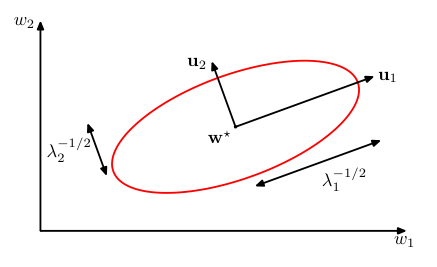
\includegraphics[width=0.6\textwidth]{figure7-2.png}
    \caption{误差函数的等值线}
\end{figure}

Figure 7.2 Caption: In the neighbourhood of a minimum $w^*$, the error function can be approximated by a quadratic. Contours of constant error are then ellipses whose axes are aligned with the eigenvectors $\mathbf{u}_i$ of the Hessian matrix, with lengths that are inversely proportional to the square roots of
the corresponding eigenvalues $\lambda_i$.

{\color{red}
翻译：

如果矩阵 $\mathbf{H}$ 满足：
\begin{equation}
\mathbf{v}^\mathrm{T} \mathbf{H} \mathbf{v} > 0, \qquad \text{对于所有的 } \mathbf{v} \text{ 均成立}
\tag{7.12}
\end{equation}
则称该矩阵为正定矩阵（positive definite）。

由于特征向量 $\{\mathbf{u}_i\}$ 构成一个完备集，任意向量 $\mathbf{v}$ 都可以表示为如下形式：
\begin{equation}
\mathbf{v} = \sum_i c_i \mathbf{u}_i.
\tag{7.13}
\end{equation}

根据公式 (7.8) 和 (7.9)，我们可以得到：
\begin{equation}
\mathbf{v}^\mathrm{T} \mathbf{H} \mathbf{v} = \sum_i c_i^2 \lambda_i
\tag{7.14}
\end{equation}
因此，$\mathbf{H}$ 为正定矩阵的充要条件是：它的所有特征值均为正数。

由此可知，$\mathbf{w}^*$ 为局部极小值点的充要条件是：误差函数的梯度在 $\mathbf{w}^*$ 处为零，且在 $\mathbf{w}^*$ 处计算的海森矩阵为正定矩阵。

在以特征向量 $\{\mathbf{u}_i\}$ 为基向量的新坐标系中，误差函数 $E(\mathbf{w})$ 的等高线是以原点为中心的、且与坐标轴对齐的椭圆，如图 7.2 所示。

图 2 图注：在极小值点 $w^*$ 的邻域内，误差函数可以用二次函数来近似。此时，误差的等高线为椭圆，其对称轴与海森矩阵的特征向量 $\mathbf{u}_i$ 对齐，且椭圆的轴长与对应特征值 $\lambda_i$ 的平方根成反比。
}

{\color{blue}
\underline{问：正定矩阵与误差等高线的几何直觉是什么？}

答：这段话从严格的代数角度给出了判断局部极小值的“终极法则”，并给出了非常直观的几何画面：

1. 为什么是正定矩阵？

公式 (7.14) 揭示了核心：$\mathbf{v}^\mathrm{T} \mathbf{H} \mathbf{v} = \sum_i c_i^2 \lambda_i$。
因为 $c_i^2$ 永远是大于等于 0 的，所以要想让这个求和式对于任意非零向量 $\mathbf{v}$ 都严格大于 0，唯一的办法就是所有的 $\lambda_i$（特征值）都必须是正数。这就是正定矩阵的代数本质。

2. 等高线为什么是椭圆？

回想一下我们之前推导的公式 (7.11)：$E(\mathbf{w}) = E(\mathbf{w}^*) + \frac{1}{2} \sum_i \lambda_i \alpha_i^2$。

如果我们画一条等高线（即让 $E(\mathbf{w})$ 等于某个常数），那么 $\sum_i \lambda_i \alpha_i^2$ 也必须是一个常数。

当所有的 $\lambda_i > 0$ 时，这个方程在数学上就是一个标准的多维椭球方程。

特征值 $\lambda_i$ 的大小决定了椭圆在各个轴向上的“拉伸”程度。$\lambda_i$ 越大，说明在这个方向上误差曲面的弯曲度越陡，等高线在这个方向上就被压得越扁（因为稍微偏离中心，误差就会剧烈增加）。

如果某些 $\lambda_i$ 是负数，这个方程就会变成双曲面，等高线会变成双曲线（这就是鞍点的几何特征）。

总结来说：在极小值点附近，误差曲面看起来就像一个多维的“碗”。正定矩阵保证了这个碗在任何方向上都是向上开口的，而等高线（碗底的同心圆/椭圆）完美地刻画了这个碗底的形状。

\underline{问：为什么是“与平方根成反比”？}

答：结合我们上一轮推导的公式 (7.11)：$E(\mathbf{w}) = E(\mathbf{w}^*) + \frac{1}{2} \sum_i \lambda_i \alpha_i^2$。

如果我们画一条等高线（即让误差函数值 $E$ 为一个常数，那么方程变为：
$$\sum_i \lambda_i \alpha_i^2 = C$$

把它化为标准椭圆方程的形式：
$$\sum_i \frac{\alpha_i^2}{(C / \lambda_i)} = 1$$

从中可以看出，椭圆在第 $i$ 个主轴方向上的半轴长度是 $\sqrt{C / \lambda_i}$。因此，特征值 $\lambda_i$ 越大（说明该方向上曲面越陡峭），对应的半轴长度 $\frac{\sqrt{C}}{\sqrt{\lambda_i}}$ 就越短，完美印证了“轴长与特征值的平方根成反比”这一结论。

% 到这里，关于误差曲面、梯度、海森矩阵以及局部极小值判断的完整理论体系就梳理完了。
% 到这里，关于局部二次近似、海森矩阵和正定性的理论推导就非常完整了。
}

\noindent\rule{\linewidth}{0.4pt}
 

\end{document}